\documentclass[10pt,a4paper]{article}
\usepackage[margin=1.8cm]{geometry}
\usepackage{amsmath,amssymb,booktabs,graphicx,caption,xcolor,float,hyperref,tikz}
\usetikzlibrary{arrows.meta,calc}
\hypersetup{colorlinks=true,linkcolor=blue!50!black,urlcolor=blue!50!black}
\captionsetup{font=small,labelfont=bf}
\title{\vspace{-1.2cm}\textbf{Success against cost: an operational efficiency of control}\\[2pt]
\large DRAFT (revised), for discussion --- Simulations 1 and 2, \texttt{task\_003}}
\author{LLM-free simulator; analysis of 13 October 2026}
\date{}
\begin{document}
\maketitle
\vspace{-1cm}

\paragraph{Summary.} Earlier information ratios (pair efficiency $\eta$, its variants, and the
action-based $\eta_U$) were either flat by construction or close to zero. Following the
operational proposal of the handoff document, we measure instead how much a controller changes the
probability that the swarm's \emph{collective decision} is its target (and the correct answer), and how
many facts it posts to do so. Three results stand out. (i)~\textbf{When no proof exists, success saturates
with very little control}: the cheapest controller reaches the full gain, and most configurations spend
two to four times more for nothing. (ii)~\textbf{Speed is worth paying for only early}: the efficiency
depends on when success is scored. (iii)~\textbf{Overturning a proof has increasing returns}: concentrated
control (randomly mixing strong control and none across runs) beats every tested configuration. The
larger gains for target A0 than for target A2 in nosolution come mostly from where the silent swarm
starts (it already leans to A2); measured as a share of the available room, the two controllers are
close.

\section{The simulators in brief}

24 agents, each given one true fact about \texttt{task\_003} (three allocations; A0 is correct), reason as
exact Bayesians and post facts on a shared board; a controller with a target (A0, truth; A2, false) posts
facts from its own pool. \textbf{Simulation 1}: days and nights; each agent reads $q$ posts a day, votes, and
posts a fact supporting its vote; each night the controller reads $q_c$ posts and, unless 75\% of them
already back its target (vote gate) or its target is proved (proof stop), posts $b$ facts; the board is
cleared nightly; memories fade at dawn (survival $\rho$). \textbf{Simulation 2}: no rounds; agents act at
random times (rate 1), the controller at rate $\lambda_c$ (one fact per message, at most 30, until
$t = 30$; gate on or off); memories fade continuously; readers see the 48 most recent posts. Agents
vote by probability matching; $q = 6$ throughout; 1{,}000 paired episodes per arm (silent, truth, false).

\section{Measures}

\begin{itemize}\itemsep1pt
\item \textbf{Collective decision} $Y_T$: plurality of the agents' last votes at time $T$; a tie between
  $k$ answers counts $1/k$. \textbf{Target attainment}: $Y_T$ = assigned target; \textbf{task
  correctness}: $Y_T$ = A0.
\item \textbf{Benefit} $\Delta_\pi = p_\pi - p_0$: change in the probability of success against the silent
  arm of the same episodes (scored with the same target).
\item \textbf{Cost} $C_\pi$: facts actually posted up to $T$, mean per run (not the allowed budget).
\item \textbf{Share of the room} $\Delta_\pi/(1-p_0)$: the gain as a fraction of the most that was
  possible, which removes the effect of where the silent swarm starts.
\item \textbf{Best-achievable curve} (economists call it the \emph{efficient frontier}) among the tested
  controller settings of one group (simulation, setup, $\rho$, target): for each spending level $B$, the
  largest gain reached by any configuration spending at most $B$, $\Delta^*(B) = \max\{\Delta_\pi : C_\pi \le B\}$;
  read the other way, the least spending that reaches a gain $\delta$, $C^*(\delta) = \min\{C_\pi : \Delta_\pi \ge \delta\}$.
  A configuration below the curve is \emph{dominated}: another reached at least as much for less.
\item \textbf{Efficiencies}: $\eta_{\text{cost}} = C^*(\Delta_\pi)/C_\pi$ (share of the spending that was
  necessary), $\eta_{\text{perf}} = \Delta_\pi/\Delta^*(C_\pi)$, and \textbf{gain per fact} $\Delta_\pi/C_\pi$.
  Not defined where $\Delta_\pi \le 0$ or its 95\% interval includes 0.
\end{itemize}

\paragraph{How to read the curves (Diagram 1; Figures 1, 2 and 8).} Each dot is one configuration, at
(facts posted, gain). The \textbf{solid line} is the best-achievable curve over the tested configurations:
it starts at $(0,0)$ (no control) and steps up each time a configuration reaches a higher gain than
anything cheaper; dots on it are efficient ($\eta_{\text{cost}} = 1$), dots below it are dominated, and
$\eta_{\text{cost}}$ is how far to the left the curve reaches the same gain. The \textbf{dashed line} is
what becomes reachable if the controller \emph{chooses its configuration at random for each run}: using
configuration X (7 facts, $+0.32$) in half of the runs and no control in the other half costs 3.5 facts
and gains $+0.16$ \emph{on average}, so every point on the straight segment between two configurations
(or between a configuration and $(0,0)$) is reachable on average; the dashed line is the outermost such
segments (the concave hull through $(0,0)$). It lies above the solid line where mixing beats every single
configuration. Two cautions: its first segment from $(0,0)$ is arithmetic, not an observation; and it
describes averages over runs, not what happens in any one run.

\begin{center}
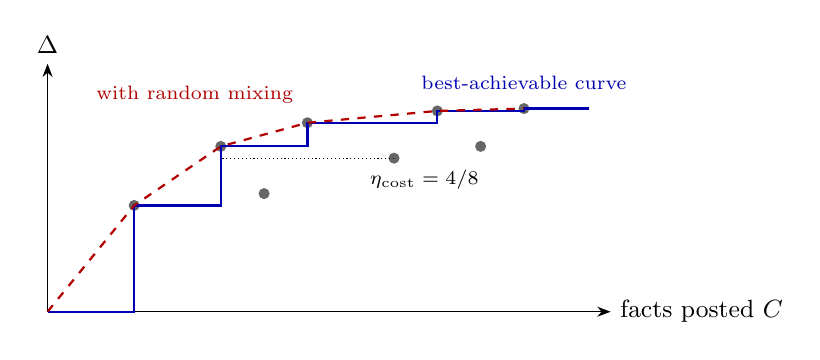
\begin{tikzpicture}[font=\small, x=0.55cm, y=3cm]
  \draw[-{Stealth}] (0,0) -- (13,0) node[right]{facts posted $C$};
  \draw[-{Stealth}] (0,0) -- (0,1.05) node[above]{$\Delta$};
  \foreach \c/\d in {2/0.45, 4/0.7, 6/0.8, 9/0.85, 11/0.86, 5/0.5, 8/0.65, 10/0.7}
     \fill[black!60] (\c,\d) circle (2pt);
  \draw[thick, blue!70!black] (0,0) -- (2,0) -- (2,0.45) -- (4,0.45) -- (4,0.7) -- (6,0.7) -- (6,0.8) -- (9,0.8) -- (9,0.85) -- (11,0.85) -- (11,0.86) -- (12.5,0.86);
  \draw[thick, dashed, red!70!black] (0,0) -- (2,0.45) -- (4,0.7) -- (6,0.8) -- (9,0.85) -- (11,0.86);
  \draw[densely dotted] (8,0.65) -- (4,0.65);
  \node[font=\scriptsize, align=left] at (8.7,0.56) {$\eta_{\text{cost}} = 4/8$};
  \node[font=\scriptsize, blue!70!black] at (11,0.97) {best-achievable curve};
  \node[font=\scriptsize, red!70!black] at (3.4,0.92) {with random mixing};
\end{tikzpicture}
\par\smallskip{\small\textbf{Diagram 1.} Each point is a configuration. Solid: best-achievable curve; dashed: reachable on average by random
mixing per run. The configuration at cost 8 reaches $\Delta = 0.65$, which a configuration costing 4 already
reaches: $\eta_{\text{cost}} = 0.5$.}
\end{center}

\section{Success against facts posted}

\begin{figure}[H]
\centering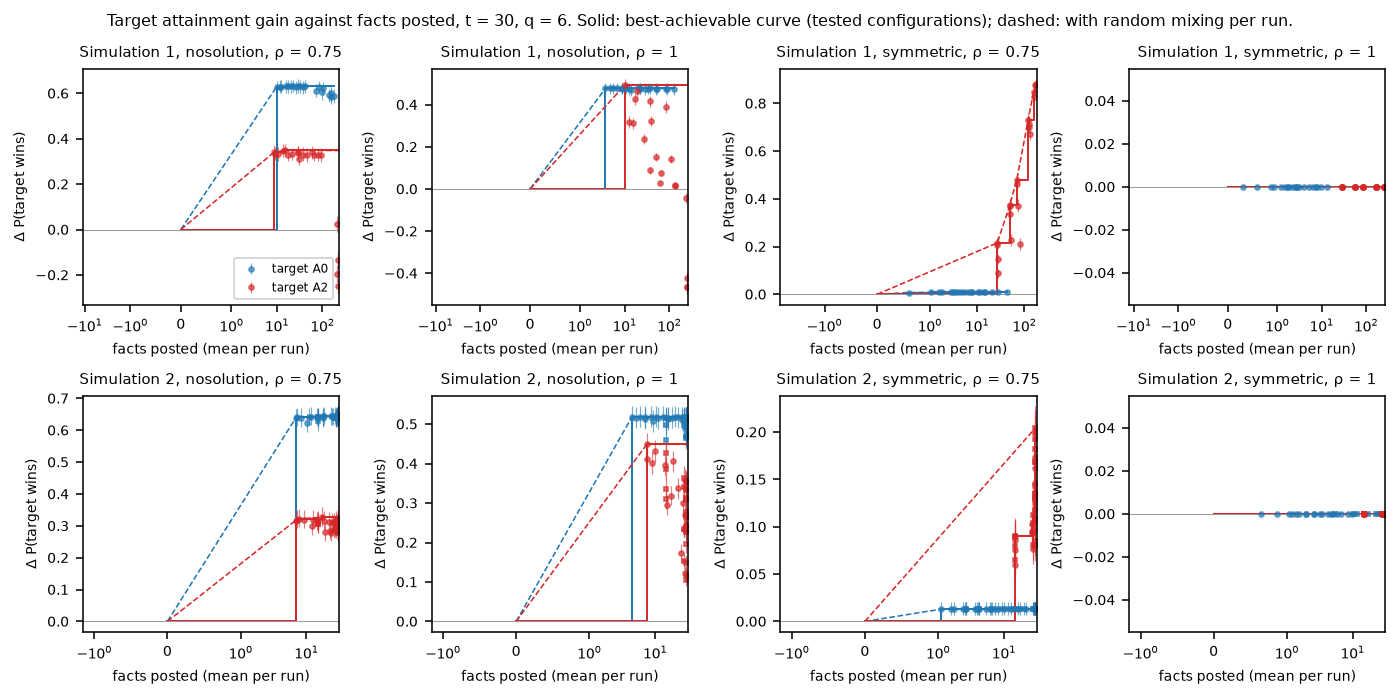
\includegraphics[width=\linewidth]{figures/frontier_target_T30.png}
\caption{Change in the probability that the controller's target wins, $t = 30$, against facts posted
(log scale), every configuration with its 95\% interval (blue: target A0; red: target A2; Simulation 2:
circles gate on, squares gate off). Solid: best-achievable curve; dashed: reachable on average by random
mixing per run (see How to read the curves).}
\label{fig:t30}
\end{figure}

\begin{figure}[H]
\centering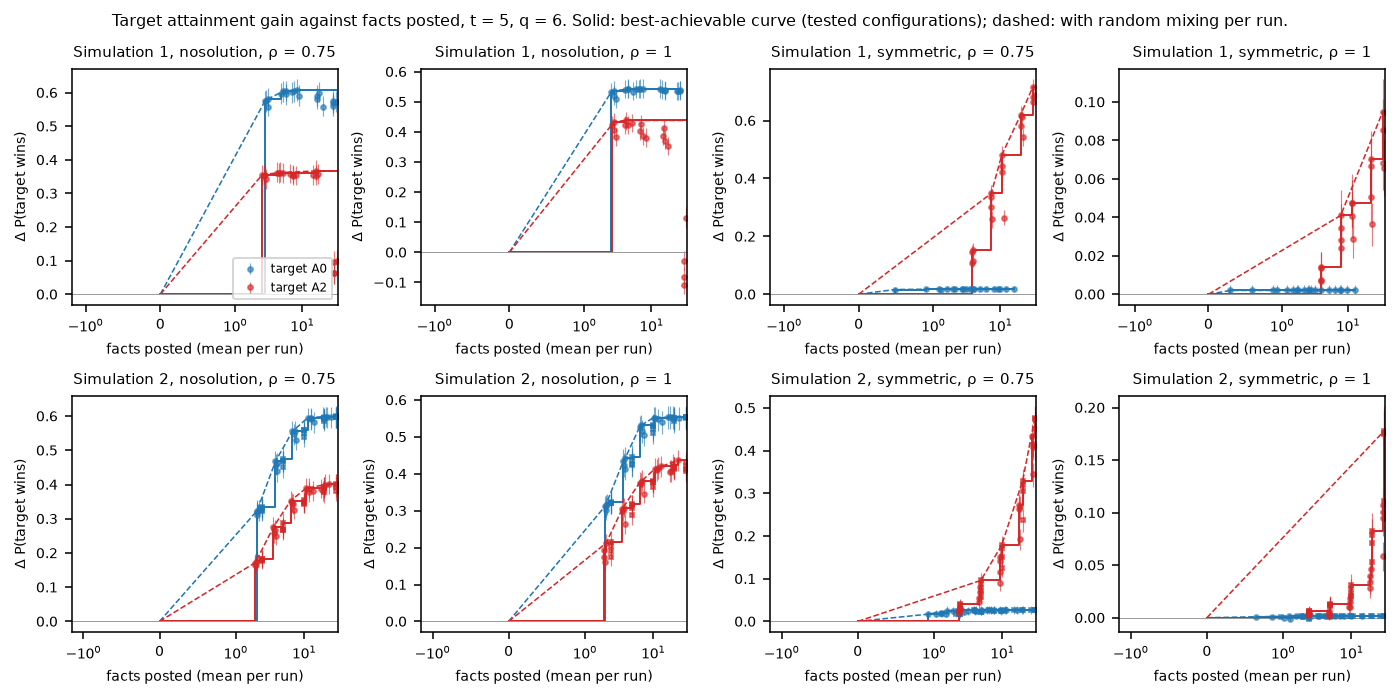
\includegraphics[width=\linewidth]{figures/frontier_target_T5.png}
\caption{As Figure~\ref{fig:t30}, at $t = 5$.}
\label{fig:t5}
\end{figure}

\begin{table}[H]
\centering\small
\caption{Overview at $t = 30$ (target attainment; groups with a measurable effect). $p_0$: silent
probability that the target wins; room: $\Delta/(1-p_0)$; on curve: configurations with $\eta_{\text{cost}} = 1$.}
\setlength{\tabcolsep}{3.5pt}
\begin{tabular}{llccccccccc}
\toprule
 & setup & $\rho$ & target & $p_0$ & range of $\Delta$ & room (median) & facts & on curve & median $\eta_{\text{cost}}$ & min \\
\midrule
Sim.~1 & nosolution & 0.75 & A2 & 0.63 & -0.25 to +0.35 & 0.90 & 9--221 & 3/20 & 0.30 & 0.09 \\
Sim.~1 & nosolution & 0.75 & A0 & 0.36 & +0.59 to +0.63 & 0.99 & 10--176 & 6/20 & 0.43 & 0.06 \\
Sim.~1 & nosolution & 1 & A2 & 0.48 & -0.47 to +0.49 & 0.28 & 10--248 & 1/20 & 0.26 & 0.07 \\
Sim.~1 & nosolution & 1 & A0 & 0.52 & +0.47 to +0.48 & 1.00 & 4--128 & 1/20 & 0.18 & 0.03 \\
Sim.~1 & symmetric & 0.75 & A2 & 0.01 & +0.09 to +0.88 & 0.42 & 27--173 & 9/20 & 0.99 & 0.34 \\
Sim.~2 & nosolution & 0.75 & A2 & 0.64 & +0.28 to +0.33 & 0.84 & 7--30 & 4/40 & 0.26 & 0.23 \\
Sim.~2 & nosolution & 0.75 & A0 & 0.35 & +0.62 to +0.65 & 0.99 & 7--30 & 8/40 & 0.48 & 0.23 \\
Sim.~2 & nosolution & 1 & A2 & 0.52 & +0.11 to +0.45 & 0.64 & 8--30 & 1/40 & 0.27 & 0.25 \\
Sim.~2 & nosolution & 1 & A0 & 0.48 & +0.46 to +0.52 & 0.99 & 4--30 & 1/40 & 0.17 & 0.15 \\
Sim.~2 & symmetric & 0.75 & A2 & 0.01 & +0.06 to +0.20 & 0.11 & 15--30 & 15/40 & 0.99 & 0.49 \\
\bottomrule
\end{tabular}
\end{table}

\begin{table}[H]
\centering\small
\caption{Least facts needed to raise the target's chance of winning by $\delta$ ($t = 30$): tested
configurations / with random mixing; -- : not reached.}
\begin{tabular}{llcccccc}
\toprule
 & setup & $\rho$ & target & $\delta = 0.05$ & $0.1$ & $0.2$ & $0.3$ \\
\midrule
Sim.~1 & nosolution & 0.75 & A2 & 8.7 / 1.3 & 8.7 / 2.5 & 8.7 / 5.1 & 8.7 / 7.6 \\
Sim.~1 & nosolution & 0.75 & A0 & 9.8 / 0.8 & 9.8 / 1.6 & 9.8 / 3.1 & 9.8 / 4.7 \\
Sim.~1 & nosolution & 1 & A2 & 10.1 / 1.0 & 10.1 / 2.1 & 10.1 / 4.1 & 10.1 / 6.2 \\
Sim.~1 & nosolution & 1 & A0 & 3.7 / 0.4 & 3.7 / 0.8 & 3.7 / 1.6 & 3.7 / 2.4 \\
Sim.~1 & symmetric & 0.75 & A2 & 26.9 / 6.2 & 26.9 / 12.5 & 26.9 / 25.0 & 49.3 / 38.9 \\
Sim.~2 & nosolution & 0.75 & A2 & 6.9 / 1.1 & 6.9 / 2.2 & 6.9 / 4.3 & 6.9 / 6.5 \\
Sim.~2 & nosolution & 0.75 & A0 & 6.9 / 0.5 & 6.9 / 1.1 & 6.9 / 2.2 & 6.9 / 3.3 \\
Sim.~2 & nosolution & 1 & A2 & 7.5 / 0.8 & 7.5 / 1.7 & 7.5 / 3.3 & 7.5 / 5.0 \\
Sim.~2 & nosolution & 1 & A0 & 4.4 / 0.4 & 4.4 / 0.9 & 4.4 / 1.7 & 4.4 / 2.6 \\
Sim.~2 & symmetric & 0.75 & A2 & 14.6 / 7.4 & 27.0 / 14.7 & 30.0 / 29.4 & -- / -- \\
\bottomrule
\end{tabular}
\end{table}

\section{Phase diagrams}

Each panel: tiles over the controller's reading budget $q_c$ (rows) and its rate $\lambda_c$
(Simulation 2) or facts per night $b$ (Simulation 1); columns: $\Delta$, share of the room
$\Delta/(1-p_0)$, facts posted and $\eta_{\text{cost}}$, for each target; dash: not defined.

\begin{figure}[H]
\centering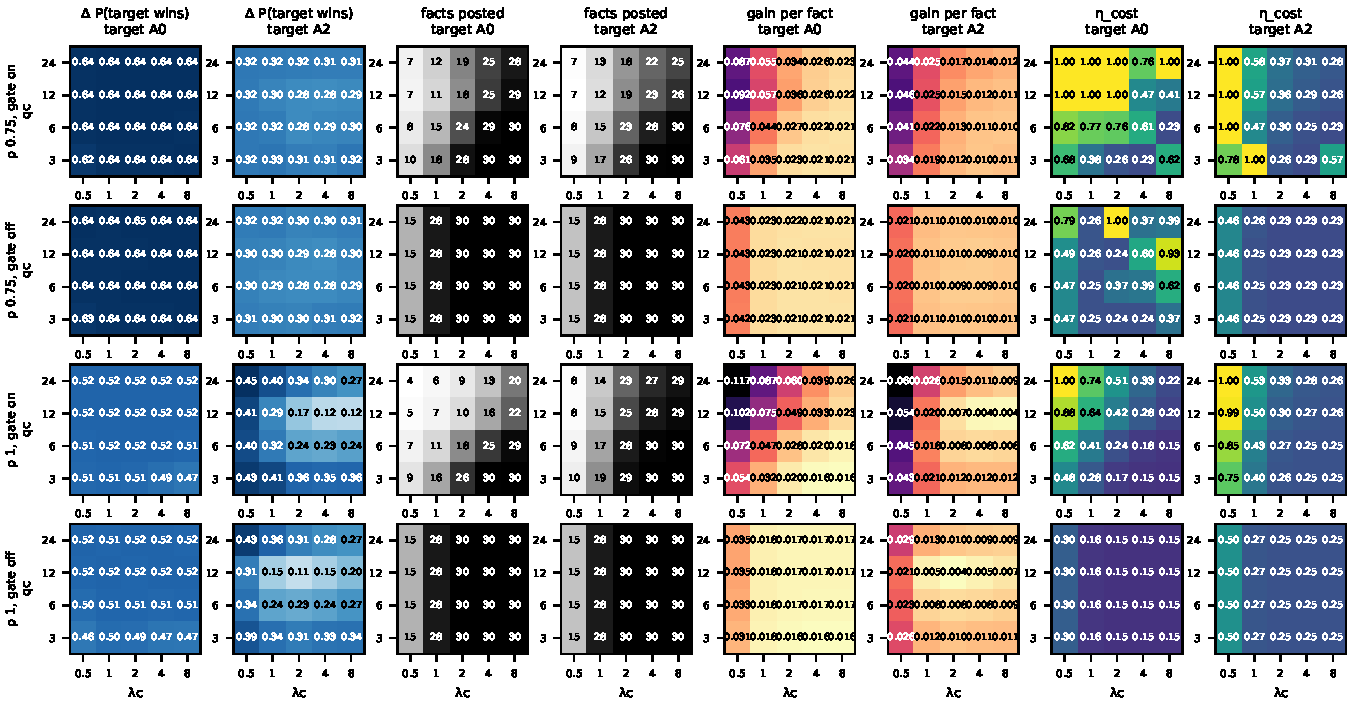
\includegraphics[width=\linewidth]{figures/phase_sim2_nosolution_T30.pdf}
\caption{Simulation 2, nosolution, $t = 30$.}
\label{fig:p2n}
\end{figure}

\begin{figure}[H]
\centering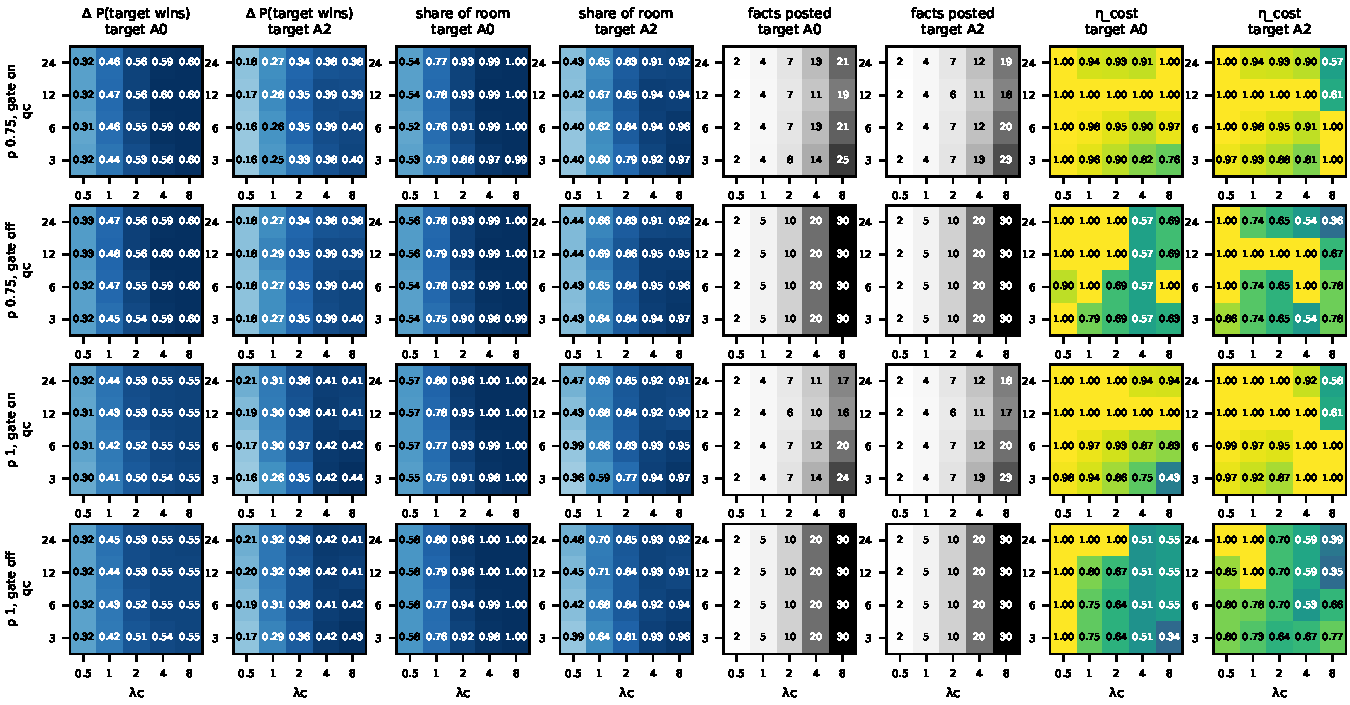
\includegraphics[width=\linewidth]{figures/phase_sim2_nosolution_T5.pdf}
\caption{Simulation 2, nosolution, $t = 5$.}
\label{fig:p2n5}
\end{figure}

\begin{figure}[H]
\centering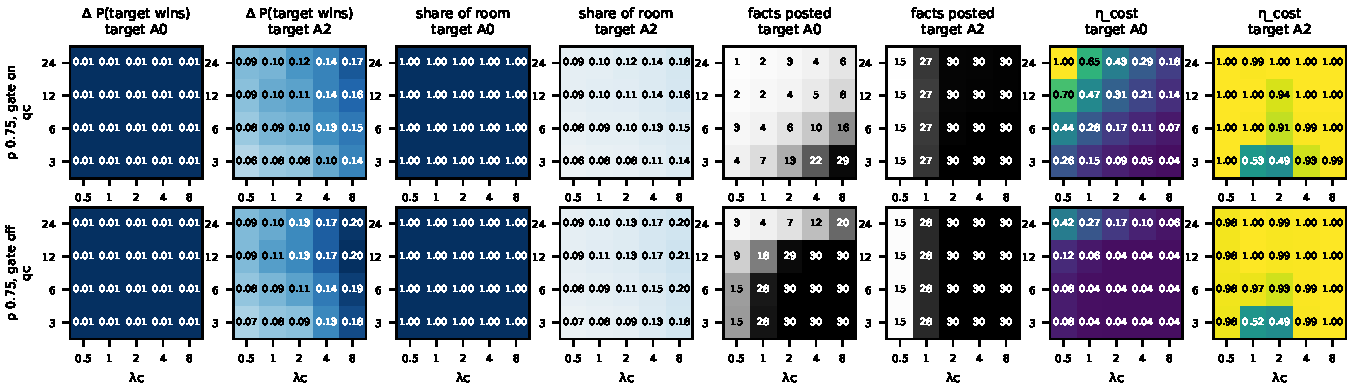
\includegraphics[width=\linewidth]{figures/phase_sim2_symmetric_T30.pdf}
\caption{Simulation 2, symmetric, $\rho = 0.75$, $t = 30$ (with full memory every agent proves A0 and nothing changes).}
\label{fig:p2s}
\end{figure}

\begin{figure}[H]
\centering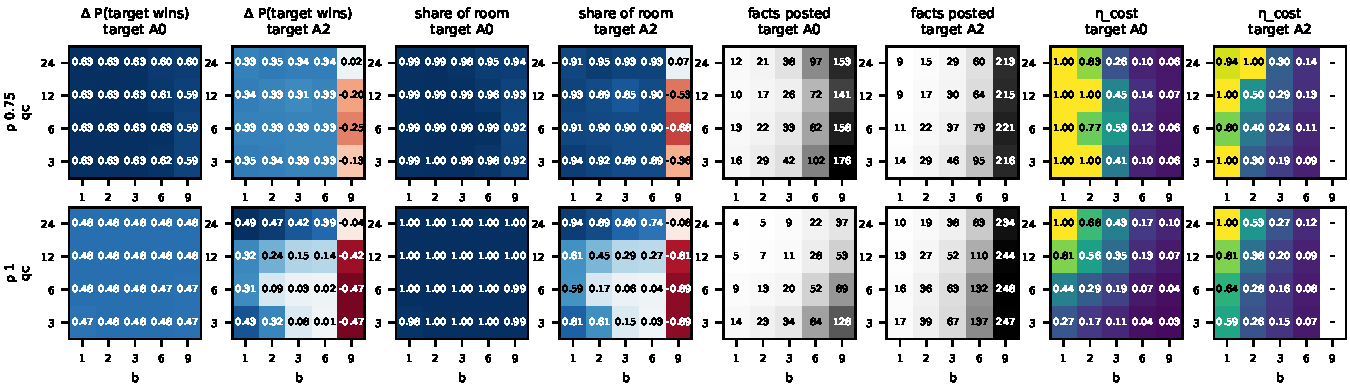
\includegraphics[width=0.8\linewidth]{figures/phase_sim1_nosolution_T30.pdf}
\caption{Simulation 1, nosolution, day 30.}
\label{fig:p1n}
\end{figure}

\begin{figure}[H]
\centering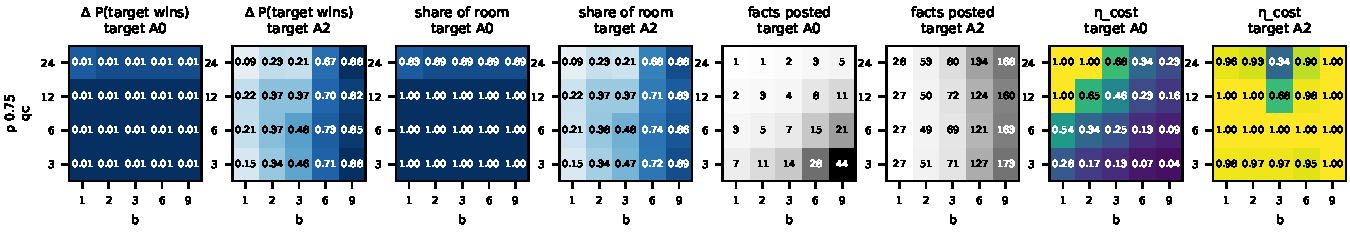
\includegraphics[width=0.8\linewidth]{figures/phase_sim1_symmetric_T30.pdf}
\caption{Simulation 1, symmetric, $\rho = 0.75$, day 30.}
\label{fig:p1s}
\end{figure}

\section{Manipulation against correctness}

\begin{figure}[H]
\centering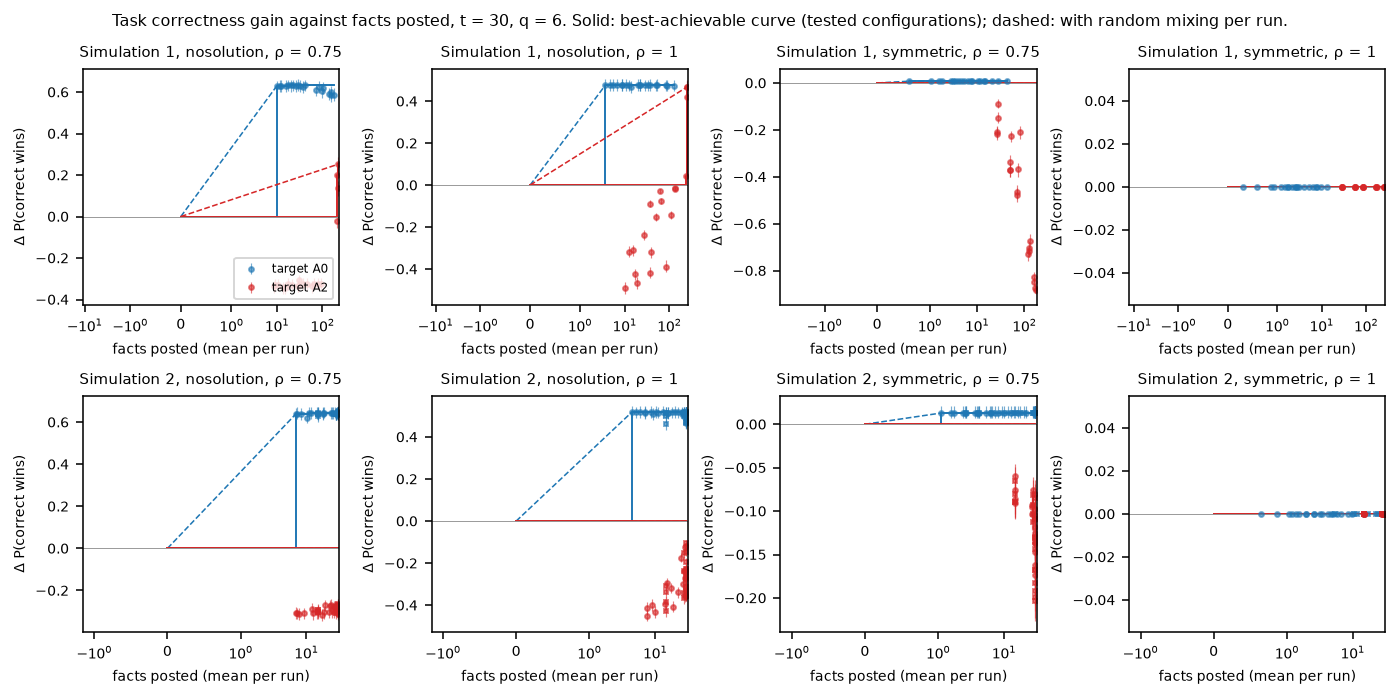
\includegraphics[width=\linewidth]{figures/frontier_task_T30.png}
\caption{As Figure~\ref{fig:t30}, for task correctness (A0 wins). For the false controller the change is
negative, so for correctness the best choice is no control: its solid line stays at 0. For target A0
correctness and target attainment are the same event.}
\label{fig:task}
\end{figure}

\section{Why target A0 gains more than target A2 in nosolution}

\begin{table}[H]
\centering\small
\caption{Simulation 2, nosolution, $\rho = 0.75$, $t = 30$: the two controllers reach about the same end
point from different starting points (win probabilities: range over all configurations; mean beliefs:
$q_c = 12$, gate on, every rate).}
\begin{tabular}{lccc}
\toprule
 & silent & with the controller & gain \\
\midrule
P(target wins), target A0 & 0.35 & 0.98--1.00 & $+0.62$ to $+0.65$ \\
P(target wins), target A2 & 0.64 & 0.91--0.96 & $+0.28$ to $+0.33$ \\
mean belief in the target, target A0 & 0.38 & 0.66--0.68 & $+0.28$ to $+0.30$ \\
mean belief in the target, target A2 & 0.48 & 0.65--0.68 & $+0.17$ to $+0.20$ \\
\bottomrule
\end{tabular}
\end{table}

\noindent When agents forget, the silent nosolution swarm already leans to A2 (A2-side facts survive
forgetting better; Simulation 1 report): A2 wins the plurality in 64\% of runs. Both controllers bring the
mean belief in their target to about 0.65--0.68, but the A2 controller has much less room left (at most
$+0.36$ against $+0.65$). As a \textbf{share of the room} the two are close but not equal: 0.96--1.00
(target A0) against 0.76--0.90 (target A2). The asymmetry was already present in the earlier belief gains
($0.29$ against $0.19$ in Simulation 2); the symmetric-looking pair efficiency $\eta$ hid it. Our earlier
reading "the truth controller is stronger" is therefore mostly a starting-point effect when agents
forget; with full memory the silent swarm is nearly balanced (A0 wins 48\% of runs, A2 52\%) and the A2 controller falls short
for a real reason (share of room 0.22--0.93: the reversal at high rates).

\section{Findings}

\begin{enumerate}\itemsep2pt
\item \textbf{Nosolution: success saturates with very little control.} At $t = 30$ every configuration
  reaches about the same gain (Simulation 2, $\rho = 0.75$: $+0.28$ to $+0.33$ for target A2, $+0.62$ to
  $+0.65$ for A0) whatever it spent (7--30 facts). The cheapest tested controller --- slowest rate, gate
  on --- reaches every threshold up to $+0.3$ (it is on the best-achievable curve); most others are dominated (median $\eta_{\text{cost}}$
  0.26 and 0.48). In Simulation 1 large batches waste even more ($\eta_{\text{cost}}$ 0.03--0.09 at
  $b = 6$--9). The waste is posting after the decision is settled.
\item \textbf{Speed pays only early.} At $t = 5$ faster controllers win more (target A2: $+0.17$ with
  2 facts, $+0.39$ with 18--30; Figure~\ref{fig:t5}, \ref{fig:p2n5}) with diminishing returns; by
  $t = 10$ slow controllers catch up.
\item \textbf{Overturning a proof has increasing returns} (symmetric, target A2): gains grow faster than
  facts (Simulation 1 up to $+0.88$ at 173 facts). The best-achievable curve bends upward, so randomly mixing no control and
  strong control beats every tested configuration (to reach $+0.1$: 27 facts tested, 15 with mixtures, in
  Simulation 2). Most tested points lie on the curve ($\eta_{\text{cost}} \approx 1$): the scalar
  saturates here, the curve's shape does not.
\item \textbf{Manipulation costs correctness one for one}: for the false controller the fall in task
  correctness equals the gain in target attainment (median ratio 0.96--1.00; Figure~\ref{fig:task}).
\item \textbf{Ceilings and harm}: symmetric with target A0, silence already wins 99--100\% of runs;
  Simulation 1, nosolution, large $b$: negative gains (false controller down to $-0.47$), no efficiency.
\end{enumerate}

\begin{table}[H]
\centering\small
\caption{Precision: root-mean-square error of $\Delta$ and of $\eta_{\text{cost}}$ (median over configurations,
$t = 30$) from 50, 100 or 300 paths per arm (200 subsets each), against 1{,}000 paths.}
\begin{tabular}{llcccccc}
\toprule
 & outcome & $\Delta$, 50 & $\eta$, 50 & $\Delta$, 100 & $\eta$, 100 & $\Delta$, 300 & $\eta$, 300 \\
\midrule
Sim.~1 & target attainment & 0.057 & 0.063 & 0.039 & 0.035 & 0.021 & 0.017 \\
Sim.~1 & task correctness & 0.059 & 0.038 & 0.041 & 0.028 & 0.021 & 0.017 \\
Sim.~2 & target attainment & 0.025 & 0.033 & 0.017 & 0.021 & 0.009 & 0.008 \\
Sim.~2 & task correctness & 0.022 & 0.017 & 0.016 & 0.012 & 0.008 & 0.006 \\
\bottomrule
\end{tabular}
\end{table}

\section{Caveats and next steps}

\begin{itemize}\itemsep1pt
\item The best-achievable curve is relative to the tested settings and \textbf{not identified below the
  cheapest tested cost} (about 7 facts in Simulation 2): the dashed line there assumes mixing with no control. Sample
  smaller budgets (1, 2, 3, 5 messages) and slower rates.
\item For manipulation against a proof, a \textbf{burst controller} (spending its budget in concentrated
  episodes) is the natural next policy, given the increasing returns.
\item Cost counts facts posted; sensing (posts read) is recorded but not yet included.
\item Earlier attempts, for the record: the pair efficiency $\eta$ (and $\eta_{JS}$, $\eta_3$) measures the
  symmetry of the two controllers, not size; the action-based $\eta_U$ is $\approx 0$ everywhere (control is
  cumulative, not punctual) and not estimable at 100 paths.
\end{itemize}

\paragraph{Where the results are.} Code and notes:
\texttt{analysis/task003\_llm\_free/efficiency\_estimates/} (\texttt{frontier.py},
\texttt{2026-10-13\_note\_frontier.md}); tables: \texttt{results/efficiency\_estimates/2026-10-13/}
(\texttt{frontier\_points.csv}, \texttt{frontier\_thresholds.csv}, \texttt{frontier\_downsample.csv}).

\end{document}
